%%%%%%%%%%%%%%%%%%%%%%%%%%%%%%%%%%%%%%%%%%%%%%%%%%%%%%%%%%%%%%%%%%%%%%%%%%%%%%%%%%
\begin{frame}[fragile]\frametitle{}
\begin{center}
{\Large Google ADK (Agent Development Kit)}
\end{center}
\end{frame}

%%%%%%%%%%%%%%%%%%%%%%%%%%%%%%%%%%%%%%%%%%%%%%%%%%%%%%%%%%%
\begin{frame}[fragile]\frametitle{Introduction to ADK Framework}
      \begin{itemize}
	\item ADK (Agent Development Kit) is Google's framework for building sophisticated AI agents and agentic applications
	\item Official documentation available at: \url{https://google.github.io/adk-docs/}
	\item Designed for production-ready agentic systems with focus on scalability and reliability
	\item Supports multi-agent systems, tool integration, and flexible deployment options
	\item Built on Google's Gemini models with support for multiple LLM providers
	\item Framework emphasizes type safety, async operations, and enterprise-grade features
	  \end{itemize}
\end{frame}

%%%%%%%%%%%%%%%%%%%%%%%%%%%%%%%%%%%%%%%%%%%%%%%%%%%%%%%%%%%%%%%%%%%%%%%%%%%%%%%%%%
\begin{frame}[fragile]\frametitle{Key Components}
	
		\begin{center}
		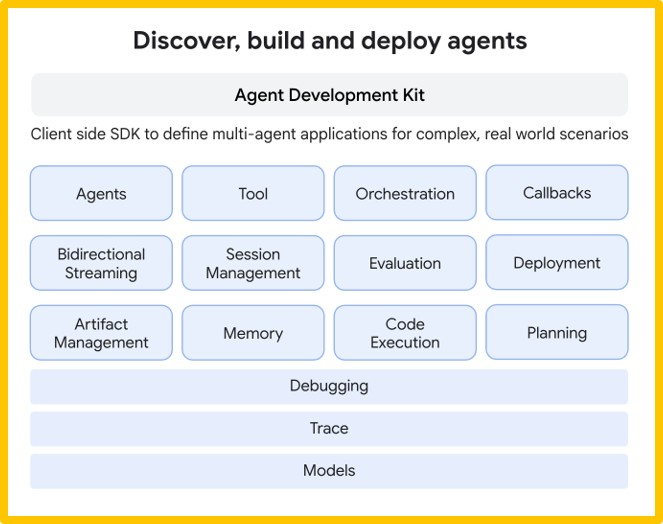
\includegraphics[width=0.8\linewidth,keepaspectratio]{aiagents127}
		
		{\tiny (Ref: Google Cloud Labgs H2 India Agents for All)}
		\end{center}	
\end{frame}

%%%%%%%%%%%%%%%%%%%%%%%%%%%%%%%%%%%%%%%%%%%%%%%%%%%%%%%%%%%
\begin{frame}[fragile]\frametitle{Key Components}

    \begin{itemize}
	\item \textbf{Agents:} Core building blocks with instructions, tools, and model configuration
	\item \textbf{Tools:} Functions that agents can call to interact with external systems and APIs
	\item \textbf{Sessions:} Manage conversation context and state across multiple interactions
	\item \textbf{Runners:} Execute agent logic with support for streaming and async operations
	\item \textbf{Memory:} Store and retrieve conversation history and context
	\item \textbf{Multi-Agent Support:} Coordinate multiple specialized agents working together
	\item \textbf{Deployment:} Built-in support for FastAPI and serverless deployment
	  \end{itemize}
\end{frame}

%%%%%%%%%%%%%%%%%%%%%%%%%%%%%%%%%%%%%%%%%%%%%%%%%%%%%%%%%%%
\begin{frame}[fragile]\frametitle{ADK Architecture Levels}
      \begin{itemize}
	\item \textbf{Basic Agents:} Single agent with tools and instructions
	\item \textbf{Stateful Agents:} Agents with session management and memory
	\item \textbf{Multi-Agent Systems:} Multiple specialized agents collaborating
	\item \textbf{Agentic Workflows:} Complex orchestration with control flow
	\item \textbf{Production Systems:} Deployed services with monitoring and scaling
	\item Each level provides additional capabilities for building sophisticated AI applications
	  \end{itemize}
\end{frame}

%%%%%%%%%%%%%%%%%%%%%%%%%%%%%%%%%%%%%%%%%%%%%%%%%%%%%%%%%%%
\begin{frame}[fragile]\frametitle{Key Features - Model Support \& Flexibility}
      \begin{itemize}
	\item \textbf{Gemini Integration:} Native support for Google's Gemini models (1.5 Pro, 2.0 Flash)
	\item \textbf{Multi-Provider:} Works with OpenAI, Anthropic, and other LLM providers
	\item \textbf{Type Safety:} Full TypeScript/Python type annotations for reliability
	\item \textbf{Async-First:} Built on async/await for high-performance concurrent operations
	\item \textbf{Streaming Support:} Real-time response streaming for better UX
	\item \textbf{Tool Calling:} Native function calling with structured input/output
	\item \textbf{Production Ready:} Built-in FastAPI integration and deployment patterns
	  \end{itemize}
\end{frame}

%%%%%%%%%%%%%%%%%%%%%%%%%%%%%%%%%%%%%%%%%%%%%%%%%%%%%%%%%%%
\begin{frame}[fragile]\frametitle{Advanced Capabilities - Grounding \& Multi-Modal}
      \begin{itemize}
	\item \textbf{Google Search Grounding:} Connect agents to real-time web search results
	\item \textbf{Multi-Modal Input:} Support for text, images, audio, and video
	\item \textbf{Code Execution:} Built-in code interpreter for dynamic computation
	\item \textbf{Vertex AI Integration:} Enterprise features like RAG and vector search
	\item \textbf{Function Calling:} Structured tool execution with automatic parameter extraction
	\item \textbf{Safety Filters:} Built-in content safety and harm prevention
	  \end{itemize}
\end{frame}

%%%%%%%%%%%%%%%%%%%%%%%%%%%%%%%%%%%%%%%%%%%%%%%%%%%%%%%%%%%
\begin{frame}[fragile]\frametitle{Enterprise Features - State \& Deployment}
      \begin{itemize}
	\item \textbf{Session Management:} Persistent conversation state across interactions
	\item \textbf{Cloud Integration:} Native support for Google Cloud services
	\item \textbf{Structured Output:} Pydantic models for type-safe responses
	\item \textbf{Error Handling:} Robust retry logic and error recovery
	\item \textbf{Monitoring:} Integration with Cloud Logging and Tracing
	\item \textbf{Authentication:} Built-in OAuth and API key management
	\item \textbf{Scalability:} Designed for high-throughput production workloads
	  \end{itemize}
\end{frame}

%%%%%%%%%%%%%%%%%%%%%%%%%%%%%%%%%%%%%%%%%%%%%%%%%%%%%%%%%%%%%%%%%%%%%%%%%%%%%%%%%%
\begin{frame}[fragile]\frametitle{Build Agents with Google Cloud-ADK}
	
		\begin{center}
		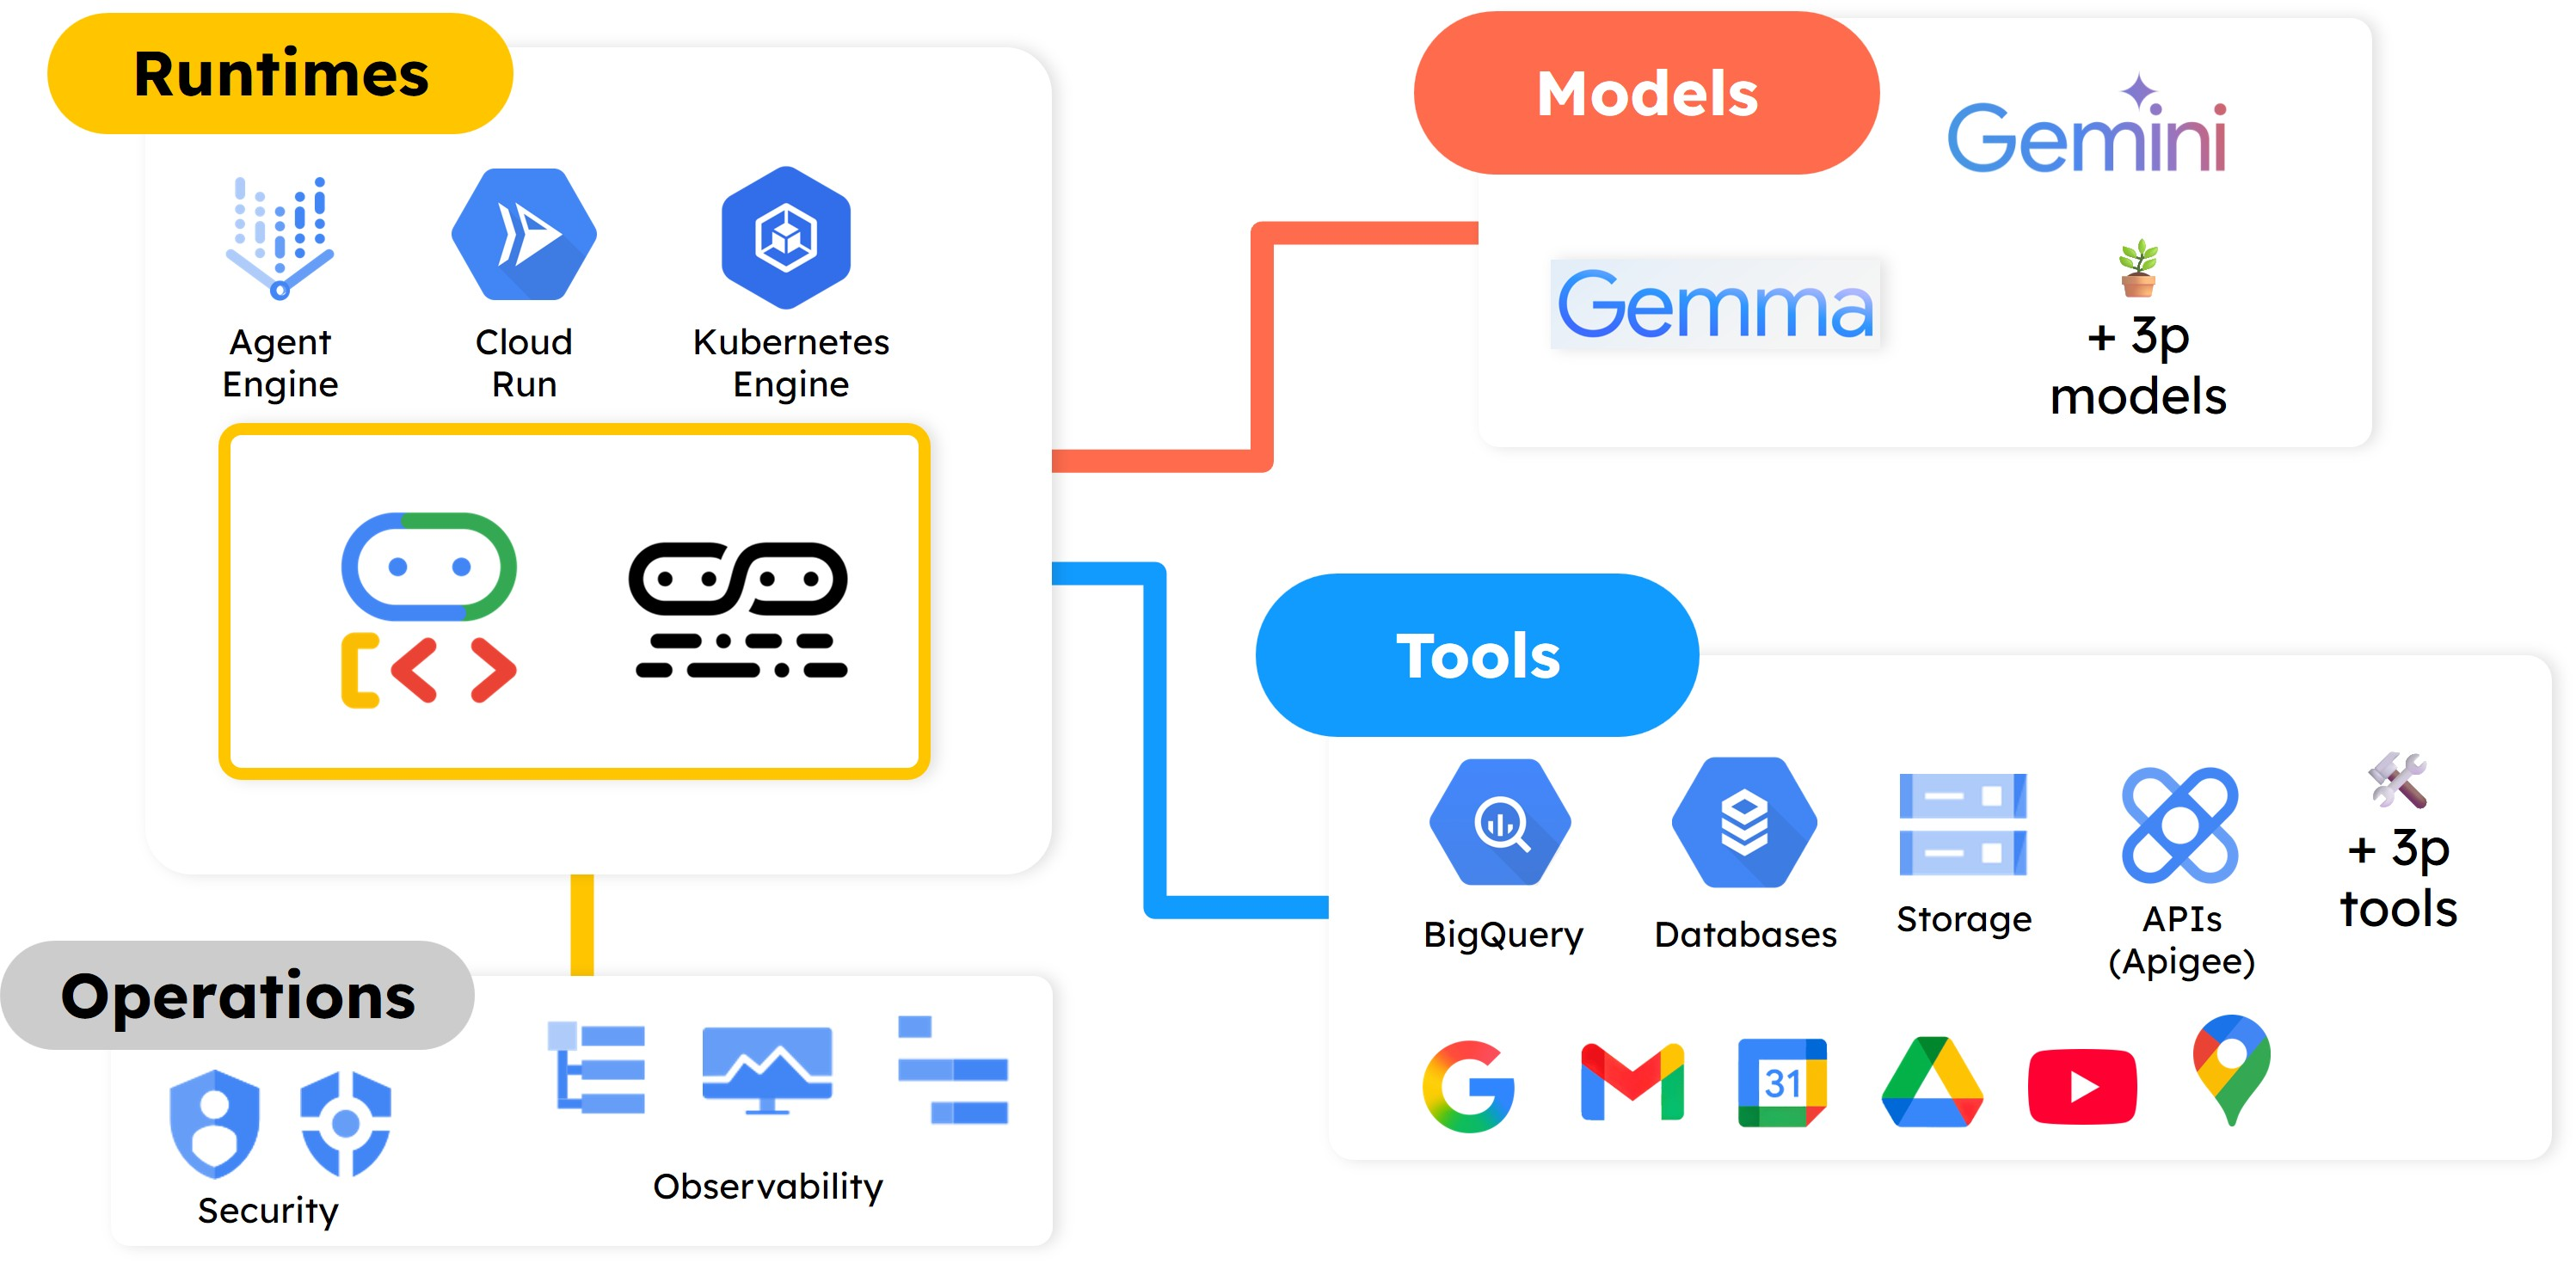
\includegraphics[width=\linewidth,keepaspectratio]{aiagents128}
		
		{\tiny (Ref: Google Cloud Labgs H2 India Agents for All)}
		\end{center}	
\end{frame}

%%%%%%%%%%%%%%%%%%%%%%%%%%%%%%%%%%%%%%%%%%%%%%%%%%%%%%%%%%%
\begin{frame}[fragile]\frametitle{Installation \& Setup}
      \begin{itemize}
	\item \textbf{Simple Installation:} Install via pip with minimal dependencies
	\item \textbf{CLI Tools:} Built-in commands for project creation and management
	\item \textbf{Project Generation:} Automatic scaffolding with best practices	
	\item \textbf{API Key Creation:}Get the API key from \url{https://aistudio.google.com/api-keys}
	\item \textbf{API Key Setup:} Configure Gemini API key via environment variable
	
	\item \textbf{Quick Start:} Start building agents immediately after installation
	  \end{itemize}
      
      \begin{lstlisting}[language=bash]
pip install google-adk
pip install google-adk --use-deprecated=legacy-resolver

# Create a new agent project
adk create my_agent

# Set API key in .env file
echo 'GOOGLE_API_KEY="YOUR_API_KEY"' > my_agent/.env # write your API key into an .env 
      \end{lstlisting}
\end{frame}

%%%%%%%%%%%%%%%%%%%%%%%%%%%%%%%%%%%%%%%%%%%%%%%%%%%%%%%%%%%
\begin{frame}[fragile]\frametitle{Use CLI not VS code}

Use Anaconda prompt with Admin permissions.

		\begin{center}
		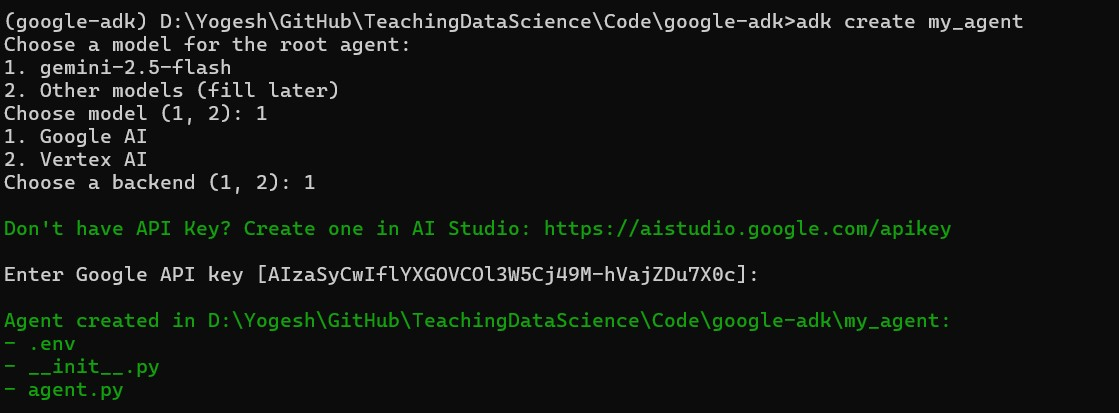
\includegraphics[width=\linewidth,keepaspectratio]{agents8}
		\end{center}	
\end{frame}
		
		
%%%%%%%%%%%%%%%%%%%%%%%%%%%%%%%%%%%%%%%%%%%%%%%%%%%%%%%%%%%
\begin{frame}[fragile]\frametitle{Explore the agent project}
      \begin{itemize}
	\item The created agent project has the following structure, with the agent.py file containing the main control code for the agent.
		\item The agent.py file contains a root\_agent definition which is the only required element of an ADK agent. You can also define tools for the agent to use. Update the generated agent.py 
		\item Run your agent using the adk run command-line tool.
		\item The ADK framework provides web interface you can use to test and interact with your agent.
	  \end{itemize}
      
      \begin{lstlisting}[language=bash]
my_agent/
    agent.py      # main agent code
    .env          # API keys or project IDs
    __init__.py
	
adk run my_agent	

adk web --port 8000 my_agent
      \end{lstlisting}
\end{frame}

%%%%%%%%%%%%%%%%%%%%%%%%%%%%%%%%%%%%%%%%%%%%%%%%%%%%%%%%%%%
\begin{frame}[fragile]\frametitle{Wrong time!!}


		\begin{center}
		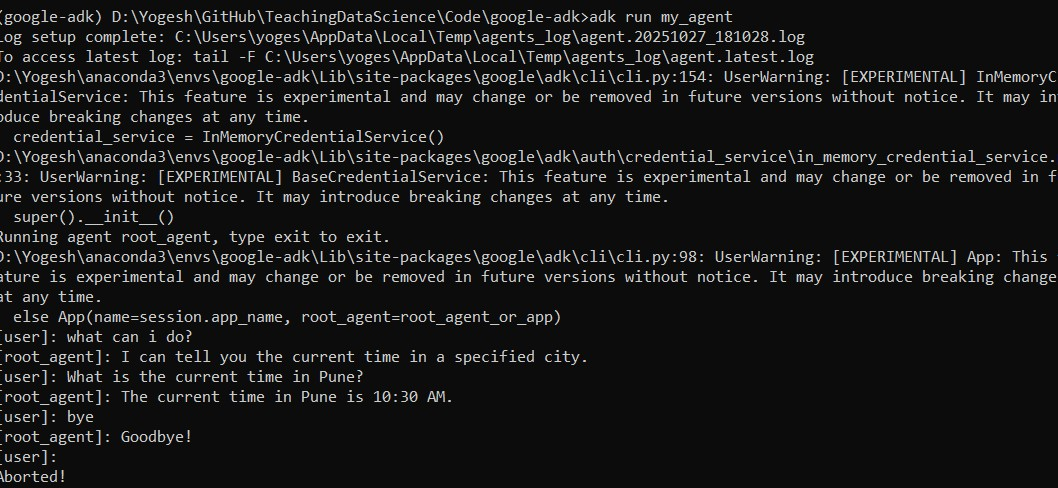
\includegraphics[width=\linewidth,keepaspectratio]{agents9}
		\end{center}	
\end{frame}

%%%%%%%%%%%%%%%%%%%%%%%%%%%%%%%%%%%%%%%%%%%%%%%%%%%%%%%%%%%
\begin{frame}[fragile]\frametitle{Basic Agent Example - Simple Setup}
      \begin{itemize}
	\item Create a basic agent with Gemini 2.0 Flash model
	\item Define tools using Python functions with type hints
	\item Agent automatically handles function calling and response generation
	\item Clean separation between tool definition and agent logic
	\item Synchronous execution for simple use cases
	  \end{itemize}
      
      \begin{lstlisting}[language=python, basicstyle=\tiny]
from adk import Agent
from adk.models import GeminiModel
import yfinance as yf

def get_stock_price(symbol: str) -> dict:
    """Get current stock price for a given symbol."""
    # Implementation using yfinance or similar
    stock = yf.Ticker(symbol)
    return {"symbol": symbol, "price": stock.info.get('currentPrice')}

agent = Agent(
    model=GeminiModel(model_name="gemini-2.0-flash-exp"),
    tools=[get_stock_price],
    instructions="You are a helpful financial assistant. Use tools when needed."
)

response = agent.run("What is NVIDIA's current stock price?")
print(response.text)
      \end{lstlisting}
\end{frame}

%%%%%%%%%%%%%%%%%%%%%%%%%%%%%%%%%%%%%%%%%%%%%%%%%%%%%%%%%%%
\begin{frame}[fragile]\frametitle{Agent with Multiple Tools}
      \begin{itemize}
	\item Define multiple specialized tools for the agent with docstring
	\item Agent selects appropriate tools based on dcostring and user query
	  \end{itemize}
      
      \begin{lstlisting}[language=python, basicstyle=\tiny]
from adk import Agent
from adk.models import GeminiModel
import yfinance as yf

def get_stock_price(symbol: str) -> float:
    """Get current stock price."""
    return yf.Ticker(symbol).info.get('currentPrice', 0)

def get_company_info(symbol: str) -> dict:
    """Get company information."""
    ticker = yf.Ticker(symbol)
    return {"name": ticker.info.get('longName'),
            "sector": ticker.info.get('sector'),
            "summary": ticker.info.get('longBusinessSummary')}

def get_analyst_recommendations(symbol: str) -> str:
    """Get analyst recommendations."""
    return yf.Ticker(symbol).recommendations.to_string()

agent = Agent(model=GeminiModel(model_name="gemini-2.0-flash-exp"),
    tools=[get_stock_price, get_company_info, get_analyst_recommendations],
    instructions="Provide detailed financial analysis using available tools.")

for chunk in agent.run_stream("Write a report on NVIDIA stock"):
    print(chunk.text, end="", flush=True)
      \end{lstlisting}
\end{frame}

%%%%%%%%%%%%%%%%%%%%%%%%%%%%%%%%%%%%%%%%%%%%%%%%%%%%%%%%%%%
\begin{frame}[fragile]\frametitle{Agent with Session Management}
      \begin{itemize}
	\item Sessions maintain conversation history and context
	\item Enable multi-turn conversations with memory
	\item Store and retrieve previous interactions
	\item Support for persistent storage backends
	  \end{itemize}
      
      \begin{lstlisting}[language=python, basicstyle=\tiny]
from adk import Agent, Session
from adk.models import GeminiModel
from adk.storage import InMemoryStorage
import yfinance as yf

def get_stock_price(symbol: str) -> float:
    """Get current stock price."""
    return yf.Ticker(symbol).info.get('currentPrice', 0)
def get_company_info(symbol: str) -> dict:
    """Get company information."""
    ticker = yf.Ticker(symbol)
    return {"name": ticker.info.get('longName'),
            "sector": ticker.info.get('sector'),
            "summary": ticker.info.get('longBusinessSummary')}
# Create storage for session history
storage = InMemoryStorage()
agent = Agent(
    model=GeminiModel(model_name="gemini-2.0-flash-exp"),
    tools=[get_stock_price, get_company_info],
    instructions="You are a financial advisor. Remember previous conversations.")
      \end{lstlisting}
\end{frame}


%%%%%%%%%%%%%%%%%%%%%%%%%%%%%%%%%%%%%%%%%%%%%%%%%%%%%%%%%%%
\begin{frame}[fragile]\frametitle{Agent with Session Management}

      \begin{lstlisting}[language=python, basicstyle=\tiny]
# Create a session for this conversation
session = Session(
    agent=agent,
    storage=storage,
    session_id="user-123"
)

# Multi-turn conversation
response1 = session.run("What's NVIDIA's stock price?")
print(response1.text)

# Agent remembers previous context
response2 = session.run("How about their competitor AMD?")
print(response2.text)

# Session history is maintained
response3 = session.run("Compare both companies")
print(response3.text)
      \end{lstlisting}
\end{frame}


%%%%%%%%%%%%%%%%%%%%%%%%%%%%%%%%%%%%%%%%%%%%%%%%%%%%%%%%%%%
\begin{frame}[fragile]\frametitle{Agent with Google Search Grounding}
      \begin{itemize}
	\item Google Search grounding provides real-time web information
	\item Automatically cites sources in responses
	\item Reduces hallucination with factual grounding
	\item Requires Vertex AI setup for production use
	  \end{itemize}
      
      \begin{lstlisting}[language=python, basicstyle=\tiny]
from adk import Agent
from adk.models import GeminiModel
from adk.extensions import GoogleSearchGrounding

agent = Agent(
    model=GeminiModel(
        model_name="gemini-2.0-flash-exp",
        extensions=[GoogleSearchGrounding()]
    ),
    instructions="Provide well-researched answers with citations."
)

response = agent.run(
    "What are the latest developments in AI semiconductor technology?"
)
print(response.text)
# Response will include citations from search results
      \end{lstlisting}
\end{frame}

%%%%%%%%%%%%%%%%%%%%%%%%%%%%%%%%%%%%%%%%%%%%%%%%%%%%%%%%%%%
\begin{frame}[fragile]\frametitle{Structured Output with Pydantic}
      \begin{itemize}
	\item Define expected output schema to ensure type-safe and structured responses
	\item Automatic validation ideal for integration with downstream systems
	  \end{itemize}
      
      \begin{lstlisting}[language=python, basicstyle=\tiny]
from adk import Agent
from adk.models import GeminiModel
from pydantic import BaseModel, Field
def get_stock_price(symbol: str) -> float:
    :
def get_company_info(symbol: str) -> dict:
    :
class StockAnalysis(BaseModel):
    symbol: str = Field(description="Stock ticker symbol")
    current_price: float = Field(description="Current stock price")
    recommendation: str = Field(description="Buy/Hold/Sell recommendation")
    reasoning: str = Field(description="Analysis reasoning")
agent = Agent(
    model=GeminiModel(model_name="gemini-2.0-flash-exp"),
    tools=[get_stock_price, get_company_info],
    output_schema=StockAnalysis,
    instructions="Analyze the stock and provide structured recommendation.")
result: StockAnalysis = agent.run("Analyze NVIDIA stock")
print(f"Symbol: {result.symbol}")
print(f"Price: ${result.current_price}")
print(f"Recommendation: {result.recommendation}")
print(f"Reasoning: {result.reasoning}")
      \end{lstlisting}
\end{frame}

%%%%%%%%%%%%%%%%%%%%%%%%%%%%%%%%%%%%%%%%%%%%%%%%%%%%%%%%%%%
\begin{frame}[fragile]\frametitle{Multi-Agent System - Architecture}
      \begin{itemize}
	\item \textbf{Specialized Agents:} Each agent focuses on specific domain expertise
	\item \textbf{Orchestration:} Coordinator agent manages task delegation
	\item \textbf{Parallel Execution:} Multiple agents can work simultaneously
	\item \textbf{Result Aggregation:} Combine outputs from multiple agents
	\item \textbf{Scalable Design:} Handle complex workflows through collaboration
	  \end{itemize}
\end{frame}

%%%%%%%%%%%%%%%%%%%%%%%%%%%%%%%%%%%%%%%%%%%%%%%%%%%%%%%%%%%
\begin{frame}[fragile]\frametitle{Multi-Agent Implementation - Part 1}
      
      \begin{lstlisting}[language=python, basicstyle=\tiny]
from adk import Agent
from adk.models import GeminiModel

def web_search(query: str) -> str:
    """Search the web for information."""
    # Implementation using search API
    pass

def get_stock_data(symbol: str) -> dict:
    """Get comprehensive stock data."""
    import yfinance as yf
    ticker = yf.Ticker(symbol)
    return {
        "price": ticker.info.get('currentPrice'),
        "recommendations": ticker.recommendations.tail(5).to_dict()
    }

web_agent = Agent(
    name="Web Agent",
    model=GeminiModel(model_name="gemini-2.0-flash-exp"),
    tools=[web_search],
    instructions="Search the web and provide sourced information."
)

finance_agent = Agent(
    name="Finance Agent",
    model=GeminiModel(model_name="gemini-2.0-flash-exp"),
    tools=[get_stock_data],
    instructions="Analyze financial data and present in clear tables."
)
      \end{lstlisting}
\end{frame}

%%%%%%%%%%%%%%%%%%%%%%%%%%%%%%%%%%%%%%%%%%%%%%%%%%%%%%%%%%%
\begin{frame}[fragile]\frametitle{Multi-Agent Implementation - Part 2}
      \begin{itemize}
	\item Coordinator agent orchestrates multiple specialized agents
	\item Delegates tasks to appropriate agents based on requirements
	\item Aggregates and synthesizes results from multiple sources
	  \end{itemize}
      
      \begin{lstlisting}[language=python, basicstyle=\tiny]
from adk import Agent, MultiAgentOrchestrator
from adk.models import GeminiModel

orchestrator = MultiAgentOrchestrator(
    agents=[web_agent, finance_agent],
    coordinator=Agent(
        model=GeminiModel(model_name="gemini-2.0-flash-exp"),
        instructions="""You coordinate a team of specialized agents.
        - Use Web Agent for market news and trends
        - Use Finance Agent for stock data and analysis
        - Synthesize their outputs into comprehensive reports.""" ))

# Run multi-agent workflow
result = orchestrator.run(
    "Provide a comprehensive analysis of AI semiconductor companies "
    "including market outlook and financial performance")

print(result.text)

# Access individual agent outputs
for agent_name, agent_result in result.agent_outputs.items():
    print(f"\n{agent_name} output:")
    print(agent_result.text)
      \end{lstlisting}
\end{frame}

%%%%%%%%%%%%%%%%%%%%%%%%%%%%%%%%%%%%%%%%%%%%%%%%%%%%%%%%%%%
\begin{frame}[fragile]\frametitle{FastAPI Deployment}
Deploy agents as REST APIs using FastAPI
      
      \begin{lstlisting}[language=python, basicstyle=\tiny]
from fastapi import FastAPI, HTTPException
from fastapi.responses import StreamingResponse
from adk import Agent, Session
from adk.models import GeminiModel
from pydantic import BaseModel
import uvicorn

app = FastAPI(title="ADK Agent API")

agent = Agent(
    model=GeminiModel(model_name="gemini-2.0-flash-exp"),
    tools=[get_stock_price, get_company_info],
    instructions="You are a financial assistant API."
)

class QueryRequest(BaseModel):
    message: str
    session_id: str

      \end{lstlisting}
\end{frame}

%%%%%%%%%%%%%%%%%%%%%%%%%%%%%%%%%%%%%%%%%%%%%%%%%%%%%%%%%%%
\begin{frame}[fragile]\frametitle{FastAPI Deployment}
     
      \begin{lstlisting}[language=python, basicstyle=\tiny]

@app.post("/chat")
async def chat(request: QueryRequest):
    session = Session(agent=agent, session_id=request.session_id)
    response = await session.run_async(request.message)
    return {"response": response.text}

@app.post("/chat/stream")
async def chat_stream(request: QueryRequest):
    session = Session(agent=agent, session_id=request.session_id)
    
    async def generate():
        async for chunk in session.run_stream_async(request.message):
            yield chunk.text
    
    return StreamingResponse(generate(), media_type="text/plain")

if __name__ == "__main__":
    uvicorn.run(app, host="0.0.0.0", port=8000)
      \end{lstlisting}
\end{frame}

%%%%%%%%%%%%%%%%%%%%%%%%%%%%%%%%%%%%%%%%%%%%%%%%%%%%%%%%%%%
\begin{frame}[fragile]\frametitle{Vertex AI Integration}
      % \begin{itemize}
	% \item Use Vertex AI for enterprise features
	% \item Vector search for RAG applications
	% \item Model deployment and versioning
	% \item Enterprise security and compliance
	  % \end{itemize}
      
      \begin{lstlisting}[language=python, basicstyle=\tiny]
from adk import Agent
from adk.models import VertexAIModel
from adk.extensions import VertexAIVectorSearch
from google.cloud import aiplatform

# Initialize Vertex AI
aiplatform.init(project="your-project-id", location="us-central1")

# Create agent with Vertex AI backend
agent = Agent(
    model=VertexAIModel(
        model_name="gemini-2.0-flash-exp",
        project="your-project-id",
        location="us-central1"
    ),
    extensions=[
        VertexAIVectorSearch(
            index_endpoint="your-index-endpoint",
            deployed_index_id="your-index-id"
        )
    ],
    instructions="Answer questions using both your knowledge and the vector store."
)

response = agent.run("What are our company policies on remote work?")
print(response.text)
      \end{lstlisting}
\end{frame}

%%%%%%%%%%%%%%%%%%%%%%%%%%%%%%%%%%%%%%%%%%%%%%%%%%%%%%%%%%%
\begin{frame}[fragile]\frametitle{Error Handling \& Reliability}
      % \begin{itemize}
	% \item Implement robust error handling for production systems
	% \item Retry logic for transient failures
	% \item Fallback mechanisms when tools fail
	% \item Logging and monitoring integration
	  % \end{itemize}
      
      \begin{lstlisting}[language=python, basicstyle=\tiny]
from adk import Agent
from adk.models import GeminiModel
from adk.exceptions import ToolExecutionError, ModelError
import logging
import yfinance as yf
logging.basicConfig(level=logging.INFO)
logger = logging.getLogger(__name__)

def safe_tool_wrapper(func):
    """Decorator for safe tool execution with fallback."""
    def wrapper(*args, **kwargs):
        try:
            return func(*args, **kwargs)
        except Exception as e:
            logger.error(f"Tool {func.__name__} failed: {e}")
            return {"error": str(e), "fallback": True}
    return wrapper

@safe_tool_wrapper
def get_stock_price(symbol: str) -> dict:
    """Get stock price with error handling."""
    return {"price": yf.Ticker(symbol).info['currentPrice']}

      \end{lstlisting}
\end{frame}


%%%%%%%%%%%%%%%%%%%%%%%%%%%%%%%%%%%%%%%%%%%%%%%%%%%%%%%%%%%
\begin{frame}[fragile]\frametitle{Error Handling \& Reliability}

      
      \begin{lstlisting}[language=python, basicstyle=\tiny]
agent = Agent(
    model=GeminiModel(
        model_name="gemini-2.0-flash-exp",
        max_retries=3,
        timeout=30
    ),
    tools=[get_stock_price],
    instructions="Handle errors gracefully and inform users."
)

try:
    response = agent.run("What's the price of NVDA?")
    print(response.text)
except ModelError as e:
    logger.error(f"Model error: {e}")
    print("Sorry, I'm having trouble processing your request.")
      \end{lstlisting}
\end{frame}

%%%%%%%%%%%%%%%%%%%%%%%%%%%%%%%%%%%%%%%%%%%%%%%%%%%%%%%%%%%
\begin{frame}[fragile]\frametitle{Framework Comparison: LangGraph vs Agno vs ADK}
\begin{table}
\tiny
\begin{tabular}{|p{2cm}|p{2cm}|p{2cm}|p{2cm}|}
\hline
\textbf{Feature} & \textbf{LangGraph} & \textbf{Agno} & \textbf{ADK} \\ \hline
\textbf{Primary Focus} & Graph-based workflows & Multi-agent systems & Enterprise AI agents \\ \hline
\textbf{Developer} & LangChain AI & Agno (ex-phidata) & Google \\ \hline
\textbf{Architecture} & State machines \& graphs & Agent teams & Agent orchestration \\ \hline
\textbf{Model Support} & 100+ providers & 23+ providers & Gemini + multi-provider \\ \hline
\textbf{Learning Curve} & Steep (graph concepts) & Moderate & Moderate \\ \hline
\textbf{Setup Time} & Complex & Minutes & Minutes \\ \hline
\textbf{Performance} & Good & 3µs instantiation & Optimized for Gemini \\ \hline
\textbf{State Management} & Built-in (checkpoints) & Session storage & Session \& Cloud \\ \hline
\textbf{Memory} & Memory modules & Built-in drivers & In-memory \& Cloud \\ \hline
\textbf{Multi-Agent} & Via subgraphs & Native teams & Orchestrator pattern \\ \hline
\textbf{Workflow Control} & Explicit graphs & Coordinate mode & Coordinator agent \\ \hline
\textbf{Streaming} & Yes & Yes & Yes (native async) \\ \hline
\textbf{RAG Support} & Vector stores & 20+ vector DBs & Vertex AI Search \\ \hline
\textbf{Deployment} & Custom & FastAPI built-in & FastAPI + Cloud Run \\ \hline
\textbf{Monitoring} & LangSmith & agno.com & Cloud Console \\ \hline
\textbf{Production Ready} & Yes & Yes & Yes (enterprise) \\ \hline
\textbf{Best For} & Complex workflows & Fast prototyping & Google Cloud users \\ \hline
\textbf{Unique Feature} & Graph visualization & 6.5KB/agent memory & Search grounding \\ \hline
\end{tabular}
\end{table}
\end{frame}

%%%%%%%%%%%%%%%%%%%%%%%%%%%%%%%%%%%%%%%%%%%%%%%%%%%%%%%%%%%
\begin{frame}[fragile]\frametitle{Best Practices}
      \begin{itemize}
	\item \textbf{Start Simple:} Begin with basic agents before adding complexity
	\item \textbf{Clear Instructions:} Provide specific, actionable instructions to agents
	\item \textbf{Tool Design:} Keep tools focused and well-documented with type hints
	\item \textbf{Error Handling:} Always implement proper error handling and retries
	\item \textbf{Testing:} Test agents thoroughly before production deployment
	\item \textbf{Monitoring:} Implement logging and monitoring for production systems
	\item \textbf{Security:} Validate inputs and sanitize outputs
	\item \textbf{Cost Management:} Monitor API usage and implement rate limiting
	  \end{itemize}
\end{frame}

%%%%%%%%%%%%%%%%%%%%%%%%%%%%%%%%%%%%%%%%%%%%%%%%%%%%%%%%%%%
\begin{frame}[fragile]\frametitle{Getting Started - Next Steps}
      \begin{itemize}
	\item \textbf{Documentation:} Explore comprehensive guides at \url{https://google.github.io/adk-docs/}
	\item \textbf{Examples Repository:} Check out example projects and templates
	\item \textbf{Community:} Join Google Cloud community for support
	\item \textbf{Start Building:} Begin with simple agents and iterate
	\item \textbf{Cloud Integration:} Leverage Google Cloud services for production
	\item \textbf{Vertex AI:} Explore enterprise features for advanced use cases
	\item \textbf{Monitoring:} Use Cloud Console for production monitoring
	  \end{itemize}
\end{frame}

%%%%%%%%%%%%%%%%%%%%%%%%%%%%%%%%%%%%%%%%%%%%%%%%%%%%%%%%%%%
\begin{frame}[fragile]\frametitle{Resources \& References}
      \begin{itemize}
	\item \textbf{Official Documentation:} \url{https://google.github.io/adk-docs/}
	\item \textbf{GitHub Repository:} \url{https://github.com/google/adk}
	\item \textbf{Gemini API:} \url{https://ai.google.dev/}
	\item \textbf{Vertex AI:} \url{https://cloud.google.com/vertex-ai}
	\item \textbf{Google Cloud:} \url{https://cloud.google.com/}
	\item \textbf{Community Support:} Google Cloud Community forums
	  \end{itemize}
\end{frame}

% %%%%%%%%%%%%%%%%%%%%%%%%%%%%%%%%%%%%%%%%%%%%%%%%%%%%%%%%%%%%%%%%%%%%%%%%%%%%%%%%%%
% \begin{frame}[fragile]\frametitle{}
% \begin{center}
% {\Large Google Agents To Agents Protocol (A2A)}
% \end{center}
% \end{frame}

% %%%%%%%%%%%%%%%%%%%%%%%%%%%%%%%%%%%%%%%%%%%%%%%%%%%%%%%%%%%
% \begin{frame}[fragile]\frametitle{References}
    % \begin{itemize}
        % \item Google ADK + A2A + MCP CRASH COURSE - The missing guide for building with its LATEST AI agent stack - AI Oriented Dev
    % \end{itemize}
% \end{frame}
